\documentclass[tikz,border=10pt]{standalone}
\usetikzlibrary{calc,intersections}
\begin{document}
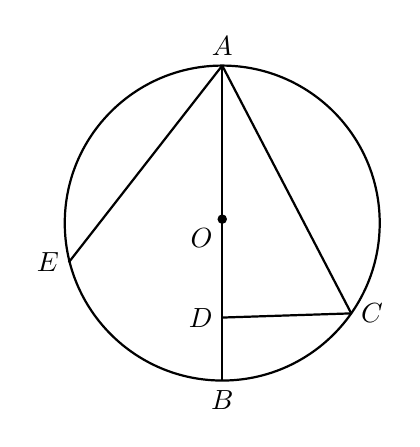
\begin{tikzpicture}    
% --- 参数定义 ---    
\def\R{2} % 圆的半径        
% --- 绘制圆 ---    
\draw[thick] (0,0) circle (\R);    
\filldraw (0,0.05) circle (1.5pt) node[below left] {$O$};        
% --- 定义关键点坐标 ---    
\coordinate (A) at (0,\R);    
\coordinate (B) at (0,-\R);    
\coordinate (C) at ({ \R*sin(55)}, {-\R*cos(55)}); % 示例坐标，可调C的位置    
\coordinate (D) at (0,{-0.6*\R}); % D点在半径上    
\coordinate (E) at (-1.95, -0.5); % E点在圆周        
% 计算M点：M是AE上一点，且OM垂直于AE    
\coordinate (M) at ($(A)!(0,0)!(E)$);        
% --- 绘制线段 ---    
\draw[thick] (A) -- (B);    
\draw[thick] (A) -- (E);    
\draw[thick] (A) -- (C);    
\draw[thick] (C) -- (D);
        % --- 标记点 ---    
\node[above] at (A) {$A$};    
\node[below] at (B) {$B$};    
\node[right] at (C) {$C$};    
\node[left] at (D) {$D$};    
\node[left] at (E) {$E$};          
% 填充及小记号    
\fill (A) circle (0pt);    
\fill (B) circle (0pt);    
\fill (C) circle (0pt);    
\fill (D) circle (0pt);    
\fill (E) circle (0pt);    
\fill (M) circle (0pt);
\end{tikzpicture}
\end{document}